\begin{figure}
    	\centering
    	\begin{minipage}{1\textwidth}
    		\centering
    		\begin{minipage}{0.45\textwidth}
    			\centering
    			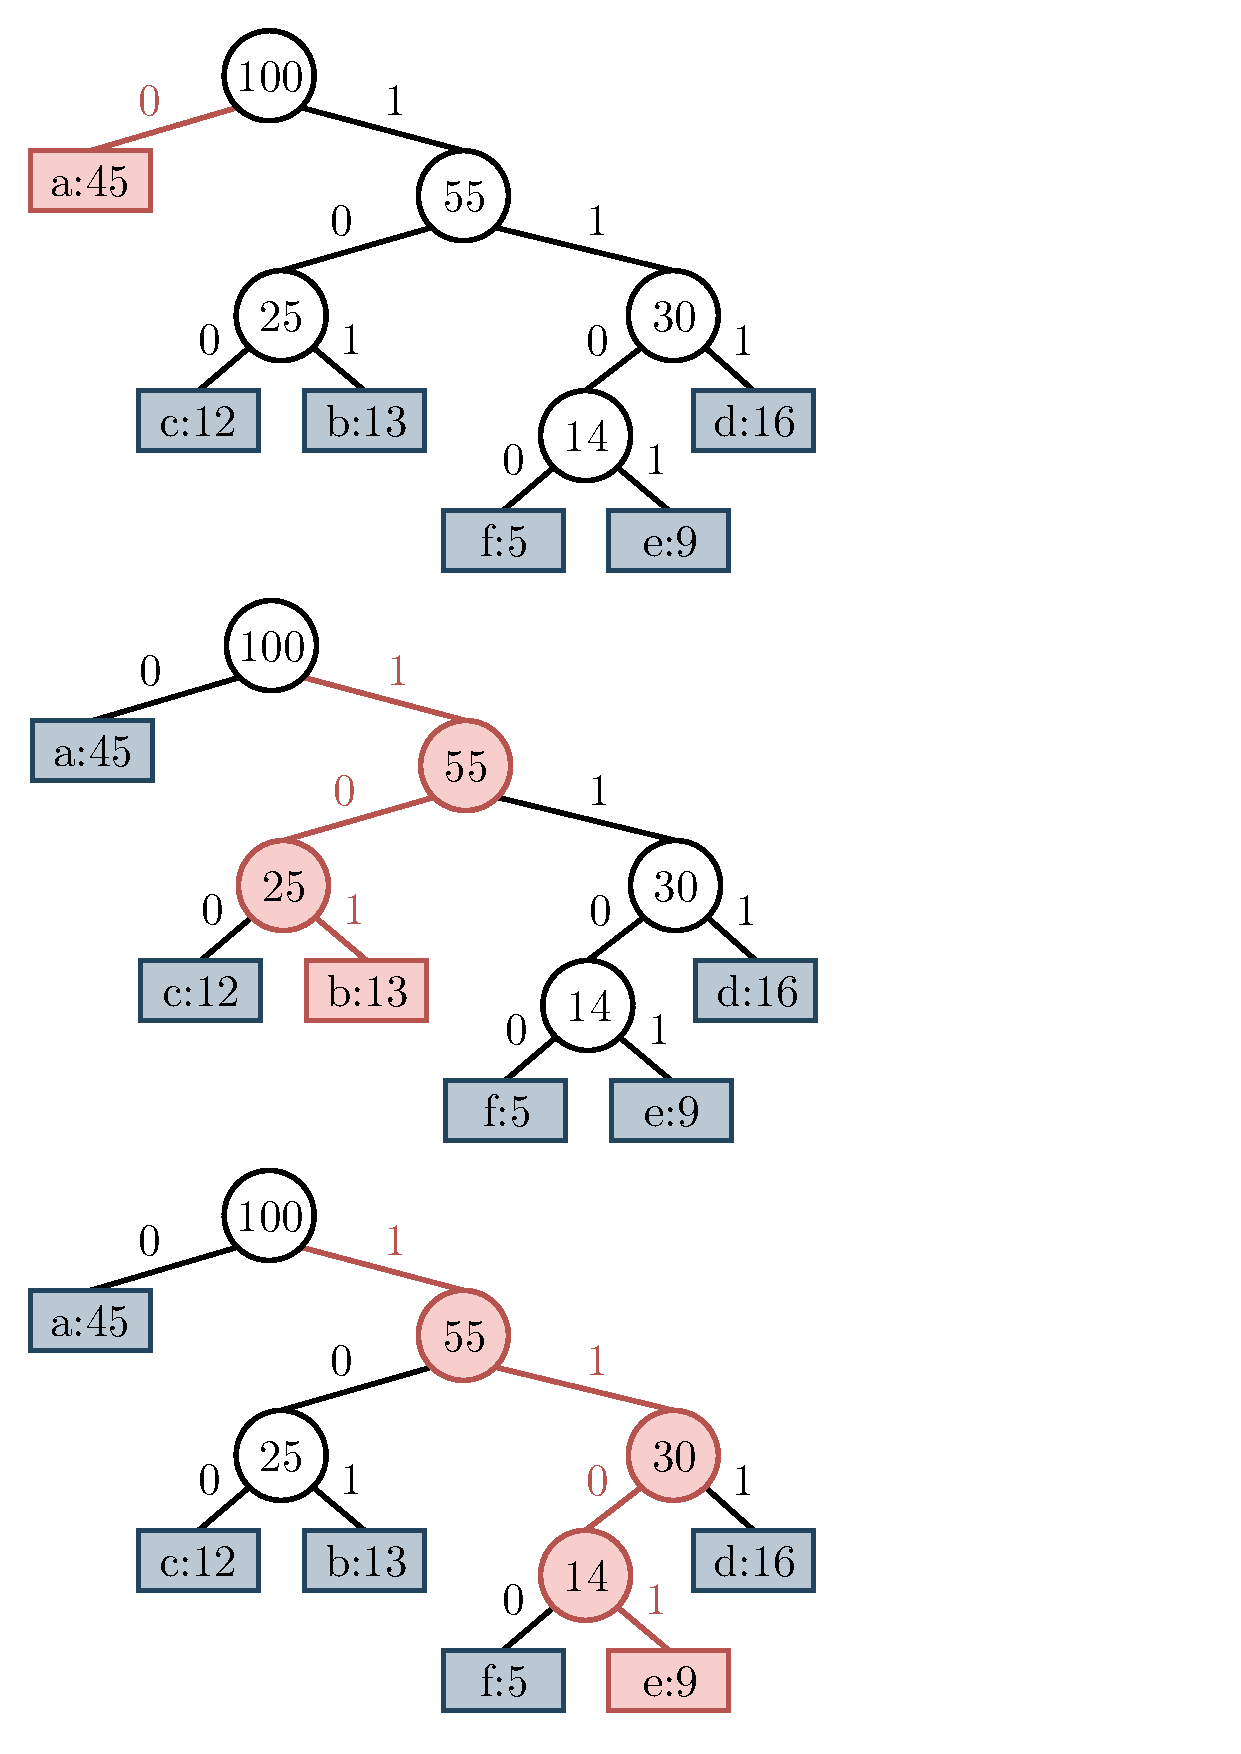
\includegraphics[scale=.45, clip, trim=10 560 200 10]{img/graphs-huffmanBack.pdf}
    			
    			(a)
    		\end{minipage}
    		\begin{minipage}{0.45\textwidth}
    			\centering
    			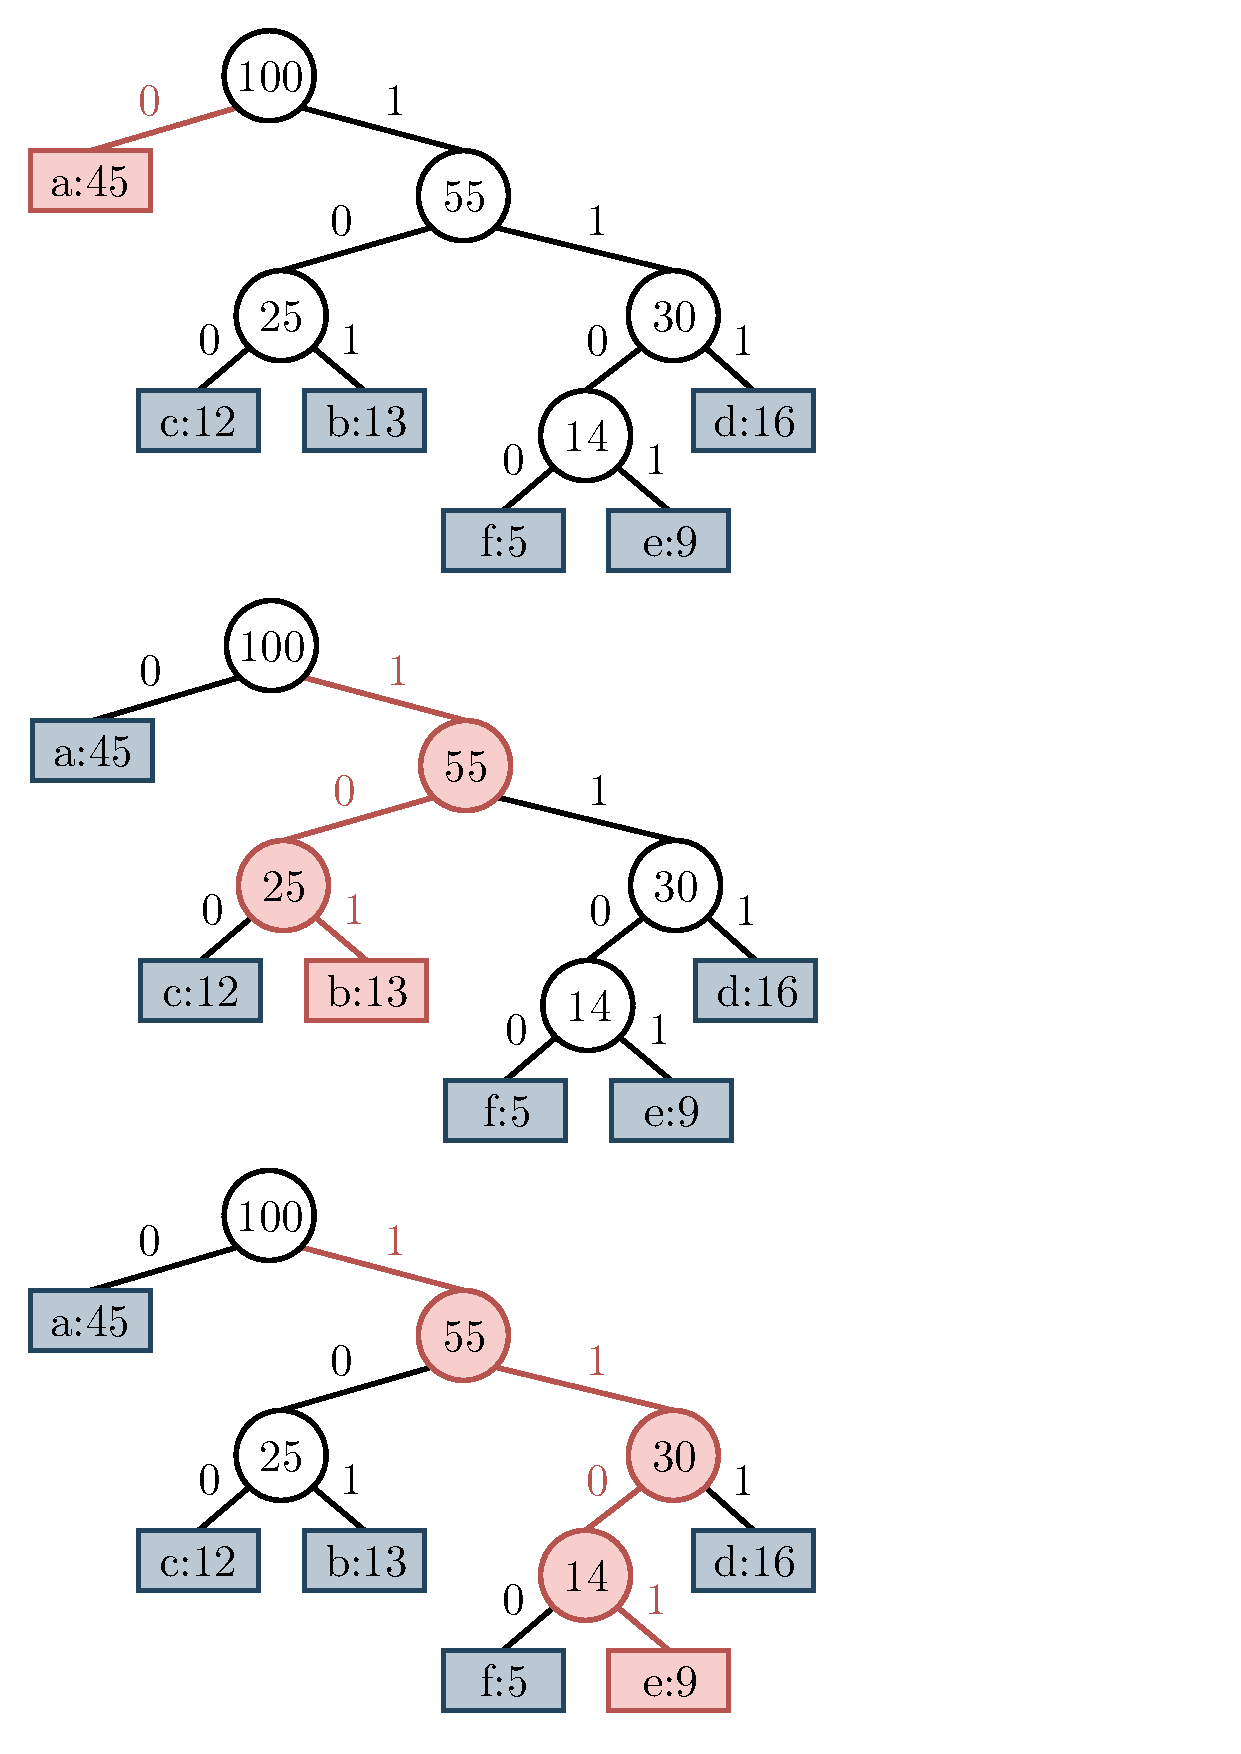
\includegraphics[scale=.45, clip, trim=10 290 200 280]{img/graphs-huffmanBack.pdf}

    			(b)
    		\end{minipage}  		
    	\end{minipage}
    	
    	\begin{minipage}{1\textwidth}
    		\centering
    		\begin{minipage}{0.45\textwidth}
    			\centering
    			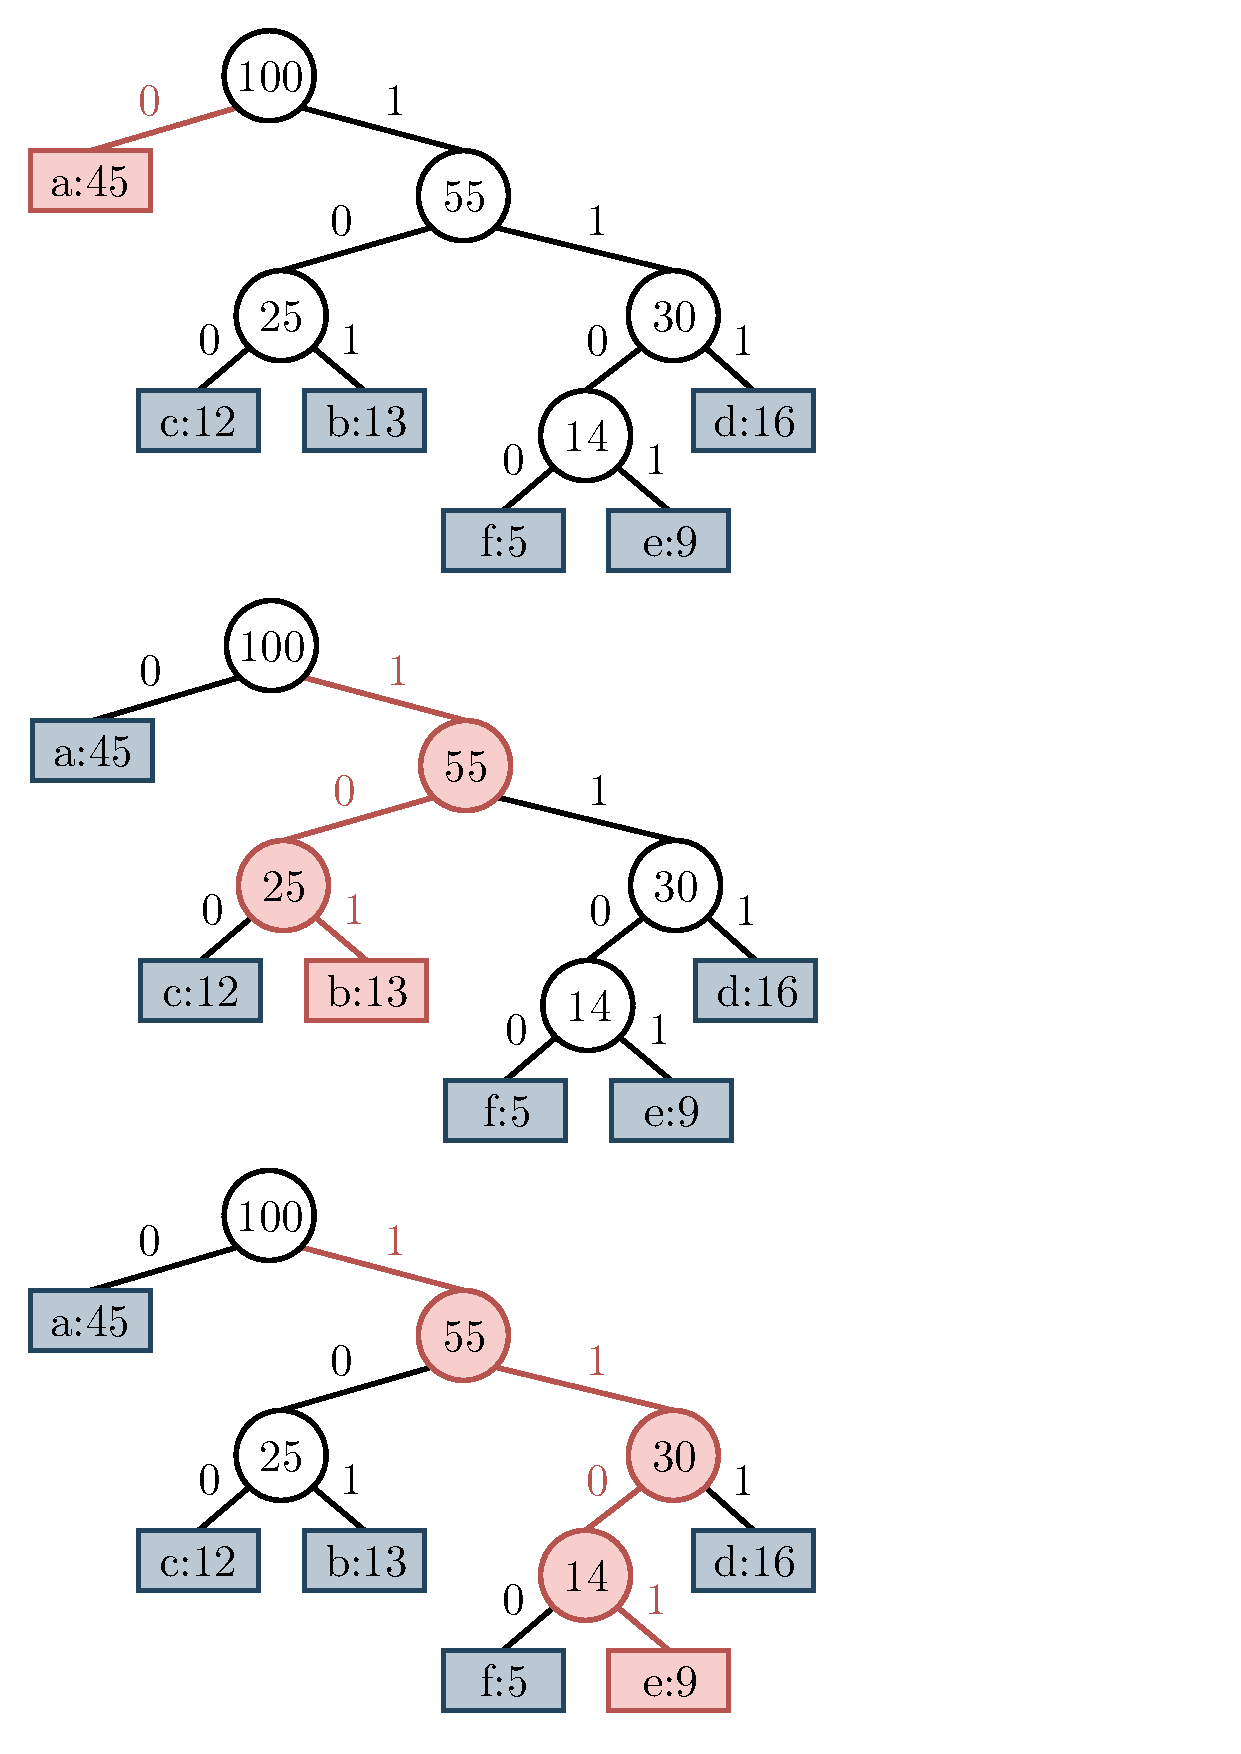
\includegraphics[scale=.4, clip, trim=10 20 200 550]{img/graphs-huffmanBack.pdf}
    			
    			(c)
    		\end{minipage}  
    		\begin{minipage}{0.45\textwidth}
    			\centering
			\begin{tabular}{cccc}
				0 & 0 & 101 & 1101 \\
				\midrule
				a & a & b & e \\
			\end{tabular}
		    	\vspace{5mm}
		    	
    			(d)
    		\end{minipage}  
    	\end{minipage}
    	
    	 
    \caption{Usando el árbol para decodificar Huffman. (a) Decodificando $0$. (b) Decodificando $101$. (c) Decodificando $1101$. (d) Equivalencias de bits y caracteres.}
    \label{fig:huffmanBack}
\end{figure}
